\chapter{Implementació com a circuit digital o en VHDL}




Sistema integrat d'emmagatzematge multiresolució de sèries temporals

  Proposta d'emmagatzematge multiresolució de sèries temporals com a
  part d'un projecte que integri xarxes de sensors.



Les xarxes de sensors capturen dades de l'entorn, les quals s'han
d'emmagatzemar en bases de dades per a poder-les tractar
posteriorment. Hi ha models que descriuen com han de ser aquestes
bases de dades per a sèries temporals i esquemes que solucionen alguns
dels seus problemes. En aquest cas, es tracta d'integrar en una xarxa
de sensors un sistema d'emmagatzematge multiresolució per a sèries
temporals.




\section{Solució d'emmagatzematge multiresolució}

Una sèrie temporal és un conjunt de parelles de temps i valor que
provenen de l'evolució d'una variable al llarg del temps. 

A causa d'aquesta naturalesa de variable capturada al llarg del temps,
en l'adquisició i tractament de les sèries temporals apareixen
propietats problemàtiques que anomenem patologies.
Algunes d'aquestes patologies són:
\begin{itemize}
\item La sincronització dels rellotges en els diferents sistemes
  d'adquisició.
\item L'aparició de dades desconegudes perquè no s'han pogut adquirir
  o perquè són errònies.
\item La gestió d'una quantitat enorme de dades i que a més segueix
  creixent al llarg del temps.
\item L'operació amb dades que no s'han recollit de manera uniforme en
  el temps.
\end{itemize}


Els sistemes informàtics que saben emmagatzemar i tractar les sèries
temporals s'anomenen sistemes de gestió de bases de dades per a sèries
temporals (SGST). Els SGST han de saber gestionar les patologies de
les sèries temporals. 

Una solució per a aquestes patologies es pot aconseguir afegint
esquemes de multiresolució per a les sèries temporals. Aleshores
s'obtenen SGST específics anomenats SGST multiresolució (SGSTM).  La
multiresolució és un sistema d'emmagatzematge que selecciona la
informació prèviament a ser guardada i en descarta la que no es
considera important.


\begin{figure}[tp]
\centering
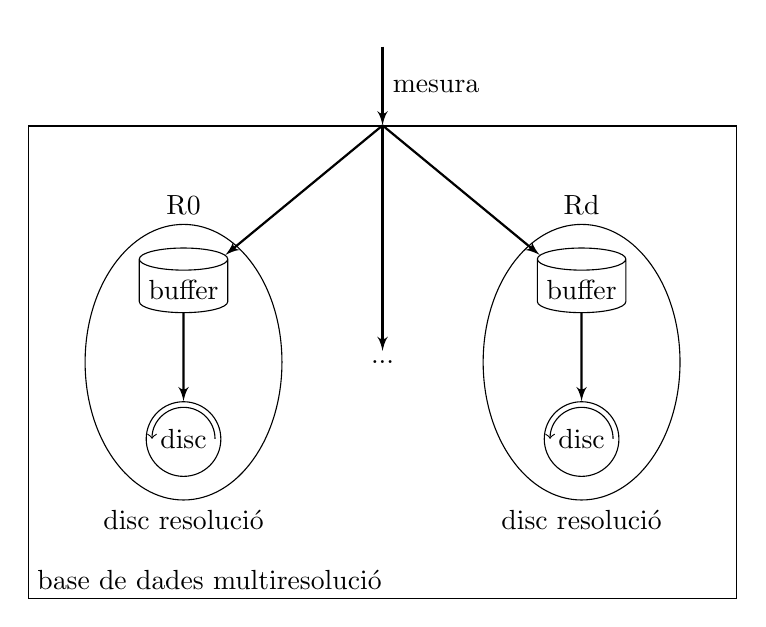
\begin{tikzpicture}
 \tikzset{
        myarrow/.style={->, >=latex',  thick},
      }
      

  \node[rectangle,draw,minimum height=6cm,minimum width=9cm] (m) {};
  \draw[shift=( m.south west)]   
  node[above right] {base de dades multiresolució};


  %discmig
  \node (m.center) (discr1) {...};

  %discr
  
  \node[ellipse,draw,minimum height=3.5cm,minimum width=2.5cm,alias=discr0] [left=of discr1] {};
  \node[above=0cm of discr0.north] {R0};
  \node[below=0cm of discr0] {disc resolució};

  \node[cylinder, draw, shape border rotate=90, aspect=0.25,alias=buffer0] [below=3mm of discr0.north] {buffer};
  \node[circle, draw,alias=disc0]  [above=3mm of discr0.south] {disc} ;
  \draw [->] (disc0.center)++(.4:.4cm) arc(0:180:.4cm);
  \draw[myarrow] (buffer0.bottom) -- (disc0.north);


  %discrd

  \node[ellipse,draw,minimum height=3.5cm,minimum width=2.5cm,alias=discrd] [right=of discr1] {};
  \node[above=0cm of discrd] {Rd};
  \node[below=0cm of discrd] {disc resolució};

  \node[cylinder, draw, shape border rotate=90, aspect=0.25,alias=bufferd] [below=3mm of discrd.north] {buffer};
  \node[circle, draw,alias=discd]  [above=3mm of discrd.south] {disc} ;
  \draw [->] (discd.center)++(.4:.4cm) arc(0:180:.4cm);
  \draw[myarrow] (bufferd.bottom) -- (discd.north);



  %mesura 
  \node[above=1cm of m.north] (m0) {};

  \draw[myarrow] (m0) -- (m.north) 
  node[right,midway] {mesura};

  \draw[myarrow] (m.north) -- (buffer0);
  \draw[myarrow] (m.north) -- (bufferd);
  \draw[myarrow] (m.north) -- (discr1);

\end{tikzpicture}
\caption{Arquitectura dels SGSTM}
\label{fig:vhdl:bdstm}
\end{figure}


Un SGSTM és una solució d'emmagatzematge per a sèries temporals a on,
resumint, la informació es distribueix mitjançant diferents
resolucions temporals.  Una sèrie temporal amb multiresolució és una
co\l.lecció de subsèries resolució, les quals acumulen temporalment
mesures en un buffer on són processades i finalment emmagatzemades
en un disc. El processament de les dades té per objectiu canviar els
intervals de temps entre les mesures per tal de compactar la
informació de les sèries temporals. D'aquesta manera, les sèries
temporals queden emmagatzemades en diferents resolucions temporals
distribuïdes en els discs.  L'arquitectura d'aquests sistemes es pot
veure a la figura~\ref{fig:vhdl:bdstm}.

Els discs tenen la mida limitada i només poden contenir un nombre
fixat de mesures. Quan un disc no té més capacitat ha d'eliminar una
mesura. Com a conseqüència en un SGSTM la mida és fixada i les sèries
temporals hi queden emmagatzemades a trossos; és a dir com a subsèries
temporals.



\section{Implementació de la multiresolució}

Els SGSTM es poden implementar amb llenguatges d'alt nivell o de baix
nivell. Cadascun ofereix avantatges i inconvenients.

Els llenguatges d'alt nivell faciliten una implementació genèrica dels
SGSTM que n'incorpori totes les capacitats i sigui totalment flexible
a nous canvis i a treballar amb varis tipus de dades. Actualment
s'està desenvolupant amb Python una implementació genèrica dels SGSTM.


En baixar de nivell es fa més difícil aconseguir implementacions
genèriques i fidedignes als models lògics, però s'aconsegueix més
especificitat i eficiència en un determinat problema i àmbit d'aplicació.

RRDtool és una implementació de SGSTM específica per a sistemes
d'adquisició de dades que provenen bàsicament de comptadors. En
aquesta implementació específica, la multiresolució té un cert esquema
prefixat i té com a avantatges l'emmagatzematge eficient al disc de les
sèries temporals i una ràpida visualització.


\section{Proposta d'implementació}

Es poden realitzar altres implementacions específiques dels SGSTM, i
és en aquest sentit que proposem l'estudi i implementació d'un SGSTM
específic en xarxes de sensors. En aquest cas es tractaria d'una
implementació en baix nivell encastada en el sensor que podria seguir
l'esquema de la figura~\ref{fig:vhdl:resolucio}, el qual és per a cada
subsèrie resolució i per tant una sèrie multiresolució estaria formada
per múltiples subsèries d'aquestes.


\begin{figure}[htp]
\centering
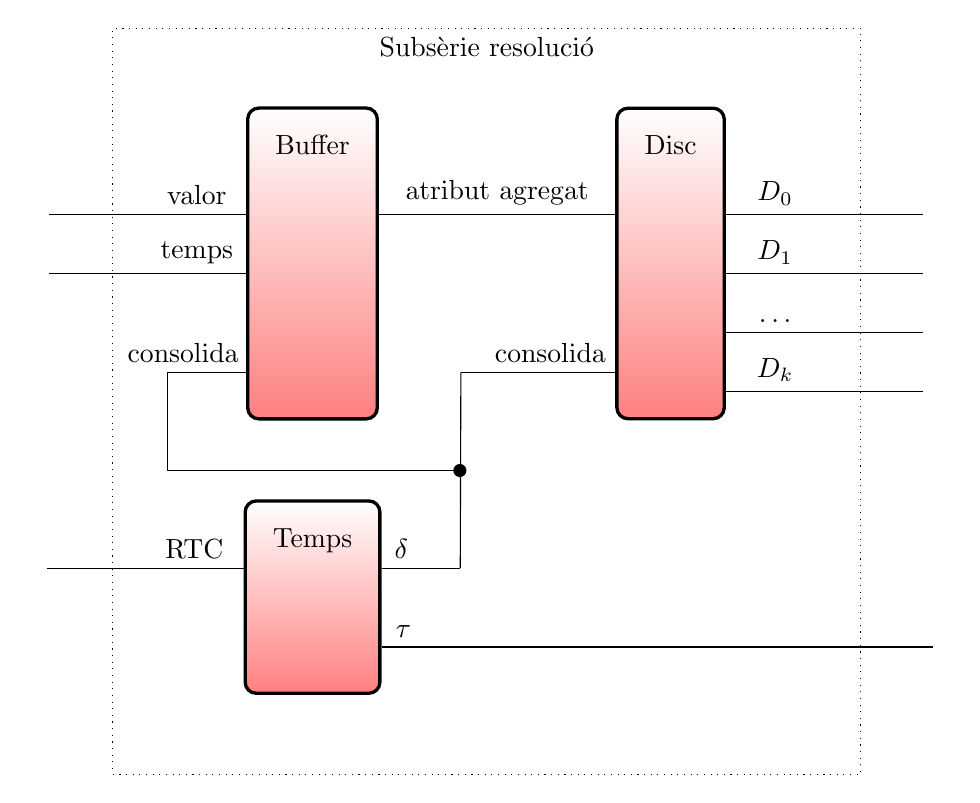
\begin{tikzpicture}
\tikzset{
    maquina/.style={rectangle,rounded corners,draw=black, 
      very thick, inner sep=1em, minimum size=3em, text centered,
      groc},
    interficie/.style={rectangle,rounded corners,draw=black, 
       inner sep=0.2em, minimum size=1em, text centered,
      verd},
    modul/.style={rectangle,rounded corners,draw=black, 
      very thick, inner sep=1em, minimum size=3em, text centered,
      roig},   
    myarrow/.style={->, >=latex', shorten >=1pt, thick},
    fletxaswitch/.style={<->, >=latex',shorten >=10pt,shorten <=10pt, thick},
    mylabel/.style={text width=7em, text centered},
    groc/.style={top color=white, bottom color=yellow!50},
    verd/.style={top color=white, bottom color=green!50},
    roig/.style={top color=white, bottom color=red!50},
  }  

  
   \node (discres) [draw, dotted, minimum width=9.5cm, text depth=9cm, rectangle] {Subsèrie resolució};



  \node[modul,text depth=3cm,below right=1cm and 1.7cm of discres.north west] (buffer) {Buffer};  

  %entrades
  \node[above left=-1.5cm and 2.5cm of buffer.north west] (buffer_valor)   {};
  \draw[-] (buffer_valor) -- (buffer_valor-|buffer.west)
   node[near end,above]{valor};

   \node[below=0.5cm of buffer_valor] (buffer_nou)   {};
   \draw[-] (buffer_nou) -- (buffer_nou-|buffer.west)
   node[near end,above]{temps};

   \node[above left=-3.5cm and 1cm of buffer.north west] (buffer_consolida) {};
   \draw[-] (buffer_consolida) -- (buffer_consolida-|buffer.west)
   node[pos=0.2,above]{consolida};

   %sortides
   \node[above right=-1.5cm and 1.5cm of buffer.north east] (buffer_dada)   {};
  \draw[-] (buffer_dada) -- (buffer_dada-|buffer.east)
   node[pos=0,above]{atribut agregat};





  \node[modul,right=3cm of buffer,text depth=3cm] (disc)   {Disc}; 

  % entrades
  \node[above left=-1.5cm and 2cm of disc.north west] (disc_valor)   {};
  \draw[-] (disc_valor) -- (disc_valor-|disc.west)
   node[near end,above]{};

  \node[above left=-3.5cm and 1.96cm of disc.north west] (disc_consolida)   {};
  \draw[-] (disc_consolida) -- (disc_consolida-|disc.west)
   node[pos=0.58,above]{consolida};

   % sortides
   \node[above right=-1.5cm and 2.5cm of disc.north east] (disc_d0)   {};
   \draw[-] (disc_d0) -- (disc_d0-|disc.east)
   node[near end,above]{$D_0$};

   \node[below=0.5cm of disc_d0] (disc_d1)   {};
  \draw[-] (disc_d1) -- (disc_d1-|disc.east)
   node[near end,above]{$D_1$};

   \node[below=0.5cm of disc_d1] (disc_d2)   {};
  \draw[-] (disc_d2) -- (disc_d2-|disc.east)
   node[near end,above]{$\dots$};

   \node[below=0.5cm of disc_d2] (disc_d3)   {};
  \draw[-] (disc_d3) -- (disc_d3-|disc.east)
   node[near end,above]{$D_k$};




  \node[modul,below=1cm of buffer,text depth=1.5cm] (temps)   {Temps}; 

  % entrades
  \node[above left=-1cm and 2.5cm of temps.north west] (temps_rtc)   {};
  \draw[-] (temps_rtc) -- (temps_rtc-|temps.west)
   node[near end,above]{RTC};

  % sortides
   \node[above right=-1cm and 1cm of temps.north east] (temps_delta)   {};
   \draw[-] (temps_delta) -- (temps_delta-|temps.east)
   node[near end,above]{$\delta$};

   \node[above right=-2cm and 7cm of temps.north east] (temps_tau)   {};
   \draw[-] (temps_tau) -- (temps_tau-|temps.east)
   node[pos=0.96,above]{$\tau$};








   %connexions
   \draw[-] (temps_delta.west) -- (disc_consolida.east); 
   
%   \node[above left=0.3cm and 1cm of temps.north west] (tau_reset)   {};
   \node[below=1cm of buffer_consolida] (tau_reset)   {};
   \draw[-*,shorten >=-2pt] (tau_reset) -- (tau_reset-|disc_consolida.east);
   \draw[-] (tau_reset.east) -- (tau_reset.east|-buffer_consolida);


 \end{tikzpicture}
 
\caption{Esquema genèric d'una subsèrie resolució}
\label{fig:vhdl:resolucio}
\end{figure}

Aquesta implementació encastada es pot realitzar tant en un
microcontrolador que emmagatzemi els valors a la memòria seguint
l'esquema de multiresolució o bé en una FPGA aprofitant que l'esquema
multiresolució té una mida finita i és per tant implementable en
hardware. 

En aquesta implementació només fem referència a la part
d'emmagatzematge. La part de tractament i consultes s'hauria de
resoldre en un sistema a part, el qual tingués més flexibilitat en el
tractament de dades. Si bé caldria implementar un protocol per tal que
aquest sistema rebés les dades emmagatzemades, el qual de forma
senzilla es podria implementar com si la base de dades multiresolució
fos un perifèric de memòria.





%\section{Aplicacions de la multiresolució en el baix nivell}




\section{MODEL}








Un disc resolució està format per un buffer, un disc i un controlador del temps.


\begin{figure}[htp]
\centering
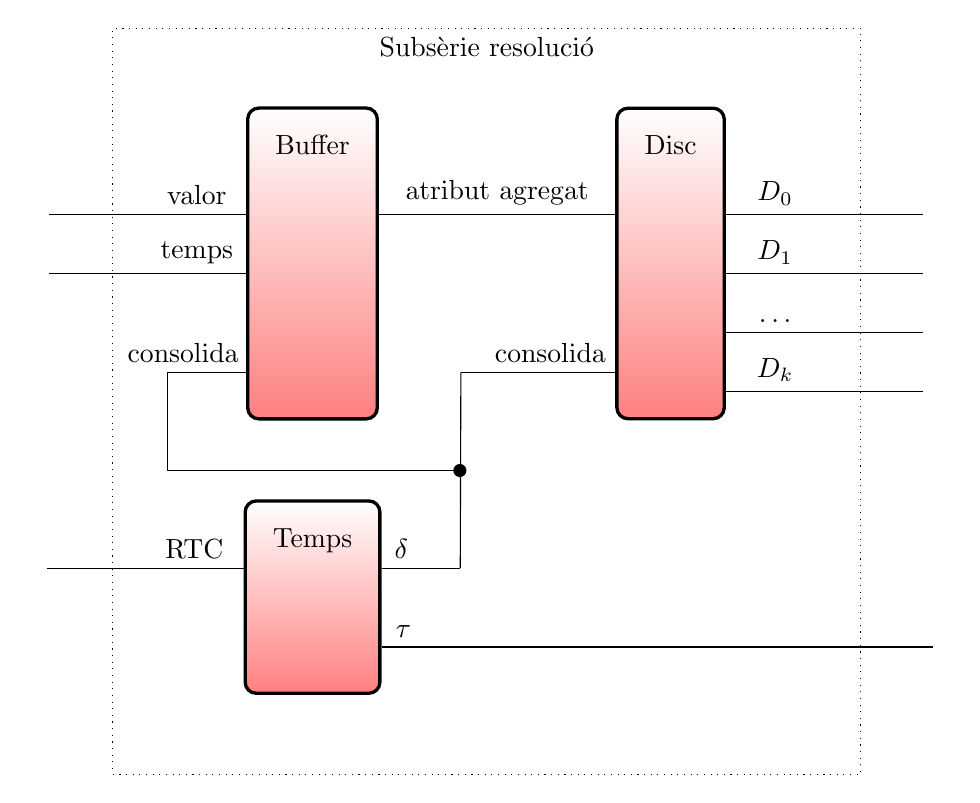
\begin{tikzpicture}
\tikzset{
    maquina/.style={rectangle,rounded corners,draw=black, 
      very thick, inner sep=1em, minimum size=3em, text centered,
      groc},
    interficie/.style={rectangle,rounded corners,draw=black, 
       inner sep=0.2em, minimum size=1em, text centered,
      verd},
    modul/.style={rectangle,rounded corners,draw=black, 
      very thick, inner sep=1em, minimum size=3em, text centered,
      roig},   
    myarrow/.style={->, >=latex', shorten >=1pt, thick},
    fletxaswitch/.style={<->, >=latex',shorten >=10pt,shorten <=10pt, thick},
    mylabel/.style={text width=7em, text centered},
    groc/.style={top color=white, bottom color=yellow!50},
    verd/.style={top color=white, bottom color=green!50},
    roig/.style={top color=white, bottom color=red!50},
  }  

  
   \node (discres) [draw, dotted, minimum width=9.5cm, text depth=9cm, rectangle] {Subsèrie resolució};



  \node[modul,text depth=3cm,below right=1cm and 1.7cm of discres.north west] (buffer) {Buffer};  

  %entrades
  \node[above left=-1.5cm and 2.5cm of buffer.north west] (buffer_valor)   {};
  \draw[-] (buffer_valor) -- (buffer_valor-|buffer.west)
   node[near end,above]{valor};

   \node[below=0.5cm of buffer_valor] (buffer_nou)   {};
   \draw[-] (buffer_nou) -- (buffer_nou-|buffer.west)
   node[near end,above]{temps};

   \node[above left=-3.5cm and 1cm of buffer.north west] (buffer_consolida) {};
   \draw[-] (buffer_consolida) -- (buffer_consolida-|buffer.west)
   node[pos=0.2,above]{consolida};

   %sortides
   \node[above right=-1.5cm and 1.5cm of buffer.north east] (buffer_dada)   {};
  \draw[-] (buffer_dada) -- (buffer_dada-|buffer.east)
   node[pos=0,above]{atribut agregat};





  \node[modul,right=3cm of buffer,text depth=3cm] (disc)   {Disc}; 

  % entrades
  \node[above left=-1.5cm and 2cm of disc.north west] (disc_valor)   {};
  \draw[-] (disc_valor) -- (disc_valor-|disc.west)
   node[near end,above]{};

  \node[above left=-3.5cm and 1.96cm of disc.north west] (disc_consolida)   {};
  \draw[-] (disc_consolida) -- (disc_consolida-|disc.west)
   node[pos=0.58,above]{consolida};

   % sortides
   \node[above right=-1.5cm and 2.5cm of disc.north east] (disc_d0)   {};
   \draw[-] (disc_d0) -- (disc_d0-|disc.east)
   node[near end,above]{$D_0$};

   \node[below=0.5cm of disc_d0] (disc_d1)   {};
  \draw[-] (disc_d1) -- (disc_d1-|disc.east)
   node[near end,above]{$D_1$};

   \node[below=0.5cm of disc_d1] (disc_d2)   {};
  \draw[-] (disc_d2) -- (disc_d2-|disc.east)
   node[near end,above]{$\dots$};

   \node[below=0.5cm of disc_d2] (disc_d3)   {};
  \draw[-] (disc_d3) -- (disc_d3-|disc.east)
   node[near end,above]{$D_k$};




  \node[modul,below=1cm of buffer,text depth=1.5cm] (temps)   {Temps}; 

  % entrades
  \node[above left=-1cm and 2.5cm of temps.north west] (temps_rtc)   {};
  \draw[-] (temps_rtc) -- (temps_rtc-|temps.west)
   node[near end,above]{RTC};

  % sortides
   \node[above right=-1cm and 1cm of temps.north east] (temps_delta)   {};
   \draw[-] (temps_delta) -- (temps_delta-|temps.east)
   node[near end,above]{$\delta$};

   \node[above right=-2cm and 7cm of temps.north east] (temps_tau)   {};
   \draw[-] (temps_tau) -- (temps_tau-|temps.east)
   node[pos=0.96,above]{$\tau$};








   %connexions
   \draw[-] (temps_delta.west) -- (disc_consolida.east); 
   
%   \node[above left=0.3cm and 1cm of temps.north west] (tau_reset)   {};
   \node[below=1cm of buffer_consolida] (tau_reset)   {};
   \draw[-*,shorten >=-2pt] (tau_reset) -- (tau_reset-|disc_consolida.east);
   \draw[-] (tau_reset.east) -- (tau_reset.east|-buffer_consolida);


 \end{tikzpicture}
 
\caption{Esquema genèric d'un disc resolució}
\label{fig:vhdl:disc-resolucio}
\end{figure}


Condicions:
\begin{itemize}
\item Àmbit: xarxes de sensors
\item No apte per processos industrials ni llaços de control, en els
  quals cal tenir totes les dades
\item Possibilitat de validació de dades del sensor (en el buffer) i
  generar avisos de funcionament incorrecte.
\item Interfície per a consulta les dades?
\end{itemize}





Estructures alternatives:
\begin{itemize}
\item timestamps absoluts: $\delta$ creats a partir de RTC
\item timestamps relatius: $\delta$ creats a partir del clock
\item timestamps creixents: l'RTC el marca el temps de la mesura
\item Memòria estàtica en comptes de volàtil. Útil per a: a) tenir dades permanents en cas d'apagada o b) per a poder consumir menys (?)   ->  tot això no seria millor fer-ho per programa (CPU) que implementat físicament (aleshores seria més reprogramable)?
\end{itemize}





Base de dades completa, conjunt de discs resolució:
\usetikzlibrary{shapes,arrows,positioning}

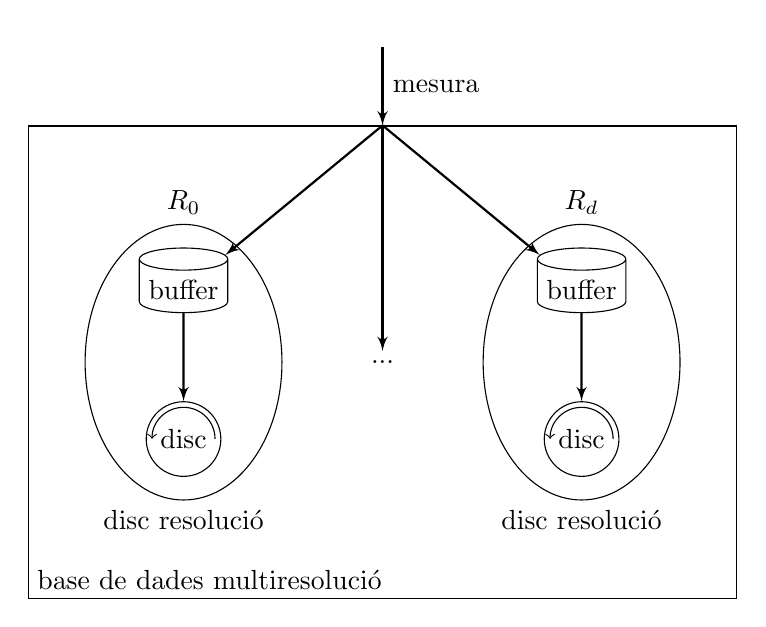
\begin{tikzpicture}
 \tikzset{
        myarrow/.style={->, >=latex',  thick},
      }
      

  \node[rectangle,draw,minimum height=6cm,minimum width=9cm] (m) {};
  \draw[shift=( m.south west)]   
  node[above right] {base de dades multiresolució};


  %discmig
  \node (m.center) (discr1) {...};

  %discr
  
  \node[ellipse,draw,minimum height=3.5cm,minimum width=2.5cm,alias=discr0] [left=of discr1] {};
  \node[above=0cm of discr0.north] {$R_0$};
  \node[below=0cm of discr0] {disc resolució};

  \node[cylinder, draw, shape border rotate=90, aspect=0.25,alias=buffer0] [below=3mm of discr0.north] {buffer};
  \node[circle, draw,alias=disc0]  [above=3mm of discr0.south] {disc} ;
  \draw [->] (disc0.center)++(.4:.4cm) arc(0:180:.4cm);
  \draw[myarrow] (buffer0.bottom) -- (disc0.north);


  %discrd

  \node[ellipse,draw,minimum height=3.5cm,minimum width=2.5cm,alias=discrd] [right=of discr1] {};
  \node[above=0cm of discrd] {$R_d$};
  \node[below=0cm of discrd] {disc resolució};

  \node[cylinder, draw, shape border rotate=90, aspect=0.25,alias=bufferd] [below=3mm of discrd.north] {buffer};
  \node[circle, draw,alias=discd]  [above=3mm of discrd.south] {disc} ;
  \draw [->] (discd.center)++(.4:.4cm) arc(0:180:.4cm);
  \draw[myarrow] (bufferd.bottom) -- (discd.north);



  %mesura 
  \node[above=1cm of m.north] (m0) {};

  \draw[myarrow] (m0) -- (m.north) 
  node[right,midway] {mesura};

  \draw[myarrow] (m.north) -- (buffer0);
  \draw[myarrow] (m.north) -- (bufferd);
  \draw[myarrow] (m.north) -- (discr1);

\end{tikzpicture}




Base de dades amb discs resolució enllaçats:

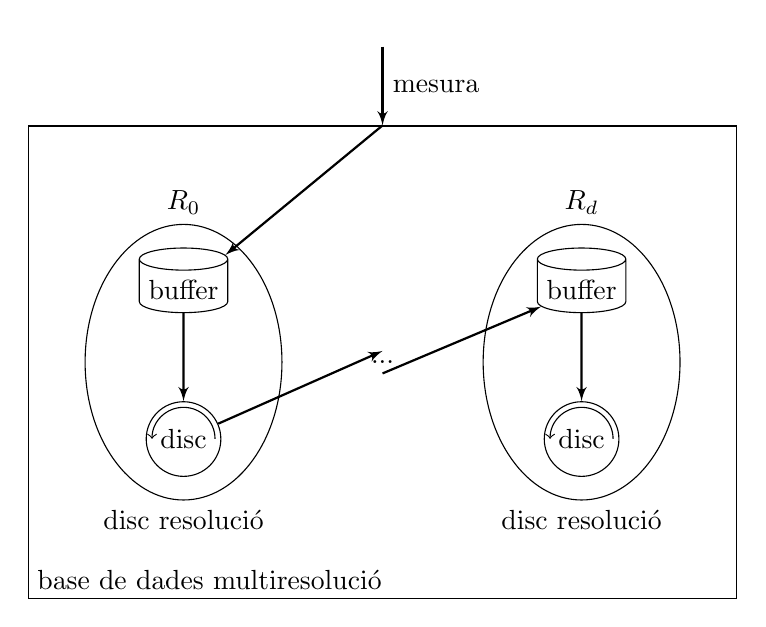
\begin{tikzpicture}
 \tikzset{
        myarrow/.style={->, >=latex',  thick},
      }
      

  \node[rectangle,draw,minimum height=6cm,minimum width=9cm] (m) {};
  \draw[shift=( m.south west)]   
  node[above right] {base de dades multiresolució};


  %discmig
  \node (m.center) (discr1) {...};

  %discr
  
  \node[ellipse,draw,minimum height=3.5cm,minimum width=2.5cm,alias=discr0] [left=of discr1] {};
  \node[above=0cm of discr0.north] {$R_0$};
  \node[below=0cm of discr0] {disc resolució};

  \node[cylinder, draw, shape border rotate=90, aspect=0.25,alias=buffer0] [below=3mm of discr0.north] {buffer};
  \node[circle, draw,alias=disc0]  [above=3mm of discr0.south] {disc} ;
  \draw [->] (disc0.center)++(.4:.4cm) arc(0:180:.4cm);
  \draw[myarrow] (buffer0.bottom) -- (disc0.north);


  %discrd

  \node[ellipse,draw,minimum height=3.5cm,minimum width=2.5cm,alias=discrd] [right=of discr1] {};
  \node[above=0cm of discrd] {$R_d$};
  \node[below=0cm of discrd] {disc resolució};

  \node[cylinder, draw, shape border rotate=90, aspect=0.25,alias=bufferd] [below=3mm of discrd.north] {buffer};
  \node[circle, draw,alias=discd]  [above=3mm of discrd.south] {disc} ;
  \draw [->] (discd.center)++(.4:.4cm) arc(0:180:.4cm);
  \draw[myarrow] (bufferd.bottom) -- (discd.north);



  %mesura 
  \node[above=1cm of m.north] (m0) {};

  \draw[myarrow] (m0) -- (m.north) 
  node[right,midway] {mesura};

  \draw[myarrow] (m.north) -- (buffer0);
  \draw[myarrow] (discr1.south) -- (bufferd);
  \draw[myarrow] (disc0) -- (discr1.north);

\end{tikzpicture}









% \begin{tikzpicture}[circuit logic IEC,
%   every circuit symbol/.style={
%     logic gate IEC symbol color=black,
%     fill=blue!20,draw=blue,very thick}]
%   \matrix[column sep=7mm]
%   {
%     \node (i0) {0}; &
%     & \\
%     & \node [and gate] (a1) {}; & \\
%     \node (i1) {0}; &
%     & \node [or gate] (o) {};\\
%     & \node [nand gate] (a2) {}; & \\
%     \node (i2) {1}; &
%     & \\
%   };
%   \draw (i0.east) -- ++(right:3mm) |- (a1.input 1);
%   \draw (i1.east) -- ++(right:3mm) |- (a1.input 2);
%   \draw (i1.east) -- ++(right:3mm) |- (a2.input 1);
%   \draw (i2.east) -- ++(right:3mm) |- (a2.input 2);
%   \draw (a1.output) -- ++(right:3mm) |- (o.input 1);
%   \draw (a2.output) -- ++(right:3mm) |- (o.input 2);
%   \draw (o.output) -- ++(right:3mm);
% \end{tikzpicture}








% \def\degr{${}^\circ$}
% \begin{tikztimingtable}
%   Clock 128\,MHz 0\degr    & H   12{2C} G \\ % ends with edge
%   Clock 128\,MHz 90\degr   & [C] 12{2C} C \\ % starts with edge
%   Clock 128\,MHz 180\degr  & C   12{2C} G \\ % ends with edge
%   Clock 128\,MHz 270\degr  &     12{2C} C \\
% \end{tikztimingtable}





\subsection{Possibles aplicacions}

Exemple d'aparell encastat molt petit, per exemple un aparell que
s'hagi de posar dins del cos per a mesurar la temperatura, a on hi ha
molt poc espai disponible i només permet emmagatzemar 100 dades. Es
poden desar 100 valors cada hora = 4 dies, o bé es pot aplicar una
solució de multiresolució i desa 75 valors cada hora = 2 dies i 25
valors cada dia = 25 dies. Així si no s'és a temps de recuperar les
dades en quatre dies sempre hi haurà alguna informació.

Exemple de la implementació de circuits integrats en materials molt prims i doblegables.




Bàsicament en les implementacions a baix nivell d'un SGSTM tenim dues opcions:

\begin{itemize}
\item implementar-ho amb llenguatge de baix nivell (assemblador, C) en un microcontrolador. Aquesta seria la manera típica perquè dóna molta flexibilitat: es pot reconfigurar l'esquema de multiresolució quan es vulgui, es poden utilitzar les operacions que es vulgui, canviar la mida, etc. 

\item implementar-ho amb hardware, per exemple dissenyar amb
  VHDL. Inconvenients: gens flexible (un cop implementat no es pot
  canviar), difícil de fer genèric (no es pot trobar un circuit que
  serveixi per a fer varis càlculs, per això caldria un
  microcontrolador). Avantatges: es pot compactar i encastar en
  llocs petits, estructures de càlcul paral·leles (la feina no recau
  en el microcontrolador), bases de dades distribuïdes. Per tant es fa
  difícil pensar de vendre BDM genèriques hardware però sí que es
  poden pensar algunes possibles aplicacions que només serien
  exclusives de hardware:

  \begin{itemize}
  \item Sensors inte\l.ligents o totalment encastats. Actualment es
    dissenyen sensors acompanyats de circuits digitals, tot encastat
    en un xip petit. Fan filtratge dels senyal, tenen un bus de
    comunicació senzill amb el controlador (I2C, 1-Wire, SPI, etc.), el
    controlador pot indicar quan s'ha d'iniciar la captura d'un no
    valor, s'emmagatzema el darrer valor capturat i el controlador el
    consulta quan vol, poden establir uns llindars d'alarma... Així
    doncs aquests sensors només emmagatzemen el darrer valor, es
    podria proposar que emmagatzemessin amb esquema multiresolució, el
    qual hauria de ser una mica configurable per exemple els períodes
    de consolidació. No obstant això, la configuració seria molt poc
    flexible i si es necessiten càlculs més complicats sempre és
    millor seguir amb l'esquema habitual del microcontrolador captura
    la dada i ell gestiona els càlculs. Ara bé, també es pot entendre
    el sensor inte\l.ligent com que forma part d'una base de dades
    distribuïda i ell té una part de l'emmagatzematge. 
    
  \item Esquema multiresolució encastat en perifèrics per a monitorar
    el seu funcionament: en una impressora en els comptadors
    d'impressions, en una antena de comunicació sense fils en els
    comptadors de bytes transmesos o la potència transmesa, etc.

  \item Implementació de circuits integrats en llocs mai vistos:
    materials molt prims i doblegables. Aquí segurament hi ha
    problemes de la mida dels circuits que es poden implementar, per
    tant poder-hi disposar d'esquemes multiresolució aniria bé.

  \item Possibilitat de disseny de FPGA casolans. Si mai això fos
    possible (sembla que ja és possible: exemple de FPGA a la
    raspberry, System-on-Chip (SoC)), els sensors intel·ligents o
    totalment encastats prendrien molt sentit ja que serien
    reconfigurables o que fos molt barat implementar en hardware un
    circuit i llençar-lo quan es volgués canviar de configuració. Això
    llavors encaixaria amb construir un xip per blocs: hi poso un bloc
    de comunicacions, un bloc de tal i un bloc de base de dades
    multiresolució amb tal esquema. Tot i així, sembla que en els SoC
    la idea és implementar-ho com a microcontrolador i fins i tot
    implementar-hi sistemes operatius.

  \item Buffers amb agregadors molt complexos: si l'agregador és complex cal implementar-ho en hardware, suposem per exemple que agrega imatge. Gestió de 1 milió de sèries temporals (article de iSAX): això com es fa? la solució podria ser sistemes hardware.


  \end{itemize}


\end{itemize}

En l'àmbit, no es veu clara la implementació de coses en VHDL. Sembla que es desaprofitar recursos perquè la feina ja la pot fer el microcontrolador. Potser l'aplicació útil i que s'ha de destacar és quan en els xips integrats no hi ha microcontrolador com poder-hi posar una base de dades?

Però sí que hi pot haver un problema de temps de computació i per tant
un aparell hardware seria necessari. Si prenem l'operació multiresolució sobre una sèrie temporal en un SGST, aquesta pot trigar molt a computar-se. Hi ha solucions en el món NoSQL, per exemple utilitzar MapReduce per a resoldre-ho en sistemes de computació para\l.lels. Però una altra solució de computació para\l.lela podria ser tenir el SGSTM implementat en hardware, aleshores aniria inserint les mesures en ordre temporal i al final obtindria el resultat; tot computat en un hardware para\l.lel. Tot i així cal notar que a més aquesta computació es pot fer en orientació stream si es coneix a priori l'operació de multiresolució que es vol fer.



%%% Local Variables:
%%% TeX-master: "main"
%%% End:
